\documentclass[border=10pt,margin=5pt,tikz,dvisvgm,rgb,utf8]{standalone}
\usepackage{ctex,xeCJK}  % 中文环境
\setCJKmainfont[BoldFont=Source Han Sans SC]{Source Han Serif SC}
\usepackage{calc,fontawesome,forest,smartdiagram,xcolor}
\usetikzlibrary{animations,arrows,automata,graphs,matrix,positioning,shadows,shapes}

\begin{document}
\renewcommand{\baselinestretch}{0.4}

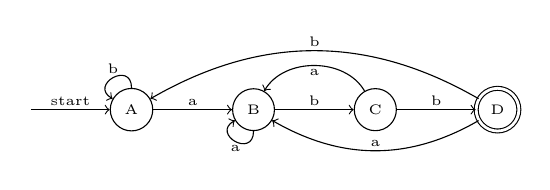
\begin{tikzpicture}
  \node[text width=-3em](start){\tiny};
  \node[circle, draw=black, right=of start](A){\tiny A};
  \node[circle, draw=black, right=of A](B){\tiny B};
  \node[circle, draw=black, right=of B](C){\tiny C};
  \node[circle, double, double distance=1pt, draw=black, right=of C](D){\tiny D};

  \path[->]
  (start) edge node[above=-2pt]{\tiny start} (A)
  (A) edge[out=90, in=150, min distance=1em] node[above=-2pt]{\tiny b} (A)
  (A) edge node[above=-2pt]{\tiny a} (B)
  (B) edge[out=270, in=210, min distance=1em] node[below=-2pt]{\tiny a} (B)
  (B) edge node[above=-2pt]{\tiny b} (C)
  (C) edge[out=120, in=60] node[below=-2pt]{\tiny a} (B)
  (C) edge node[above=-2pt]{\tiny b} (D)
  (D) edge[out=150, in=30] node[above=-2pt]{\tiny b} (A)
  (D) edge[out=210, in=330] node[above=-2pt]{\tiny a} (B);
\end{tikzpicture}

\end{document}
